\documentclass[letterpaper,11pt]{article}

\usepackage{geometry, pslatex, fancyhdr, graphicx}
\usepackage{amsmath,amsthm,amssymb,scrextend}
\usepackage{multicol}
\usepackage[makeroom]{cancel}
\usepackage{color}
\geometry{ margin = 1.0in }

%%% TODO modify these variables as per your homework %%%
\def\homeworknum{1}
\def\myname{Harshit Jain}
\def\myuserid{hmj5262}
%%%%

\pagestyle{fancy}
\lhead{{\bf CMPSC 461 Spring 2023}}
\chead{{\bf Assignment~\homeworknum}}
\rhead{{\bf \today}}
\let\newproof\proof
\renewenvironment{proof}{\begin{addmargin}[1em]{0em}\begin{newproof}}{\end{newproof}\end{addmargin}\qed}

\newcounter{problemid}
\stepcounter{problemid}
\def\newproblem{\clearpage\newpage{\bf Problem~\arabic{problemid}\stepcounter{problemid}}\hfill\par}

\setlength\parindent{0em}
\setlength\parskip{8pt}
\setlength{\fboxsep}{6pt}


\begin{document}

\framebox[\textwidth]{
	\parbox{0.96\textwidth}{
		\parbox{0.12\textwidth}{\bf Name:}\parbox{0.6\textwidth}{\myname}\\
		\parbox{0.12\textwidth}{\bf User ID:}\parbox{0.6\textwidth}{\myuserid}
	}
}
%% your solutions %%%


% PROBLEM 1
\newproblem 
\begin{enumerate}
    \item (aa)* b (bb)*?
    \item $\epsilon \mid$ a $\mid$ b $\mid$ (a $\mid$ b) (ab $\mid$ ba $\mid$ bb)
    \item (b $\mid$ ab)*a?
    \item (ab*c) $\mid$ (ba*c) $\mid$ (ac*b) $\mid$ (bc*a) $\mid$ (cb*a) $\mid$ (ca*b)
    \item It can not be constructed.
    \item \text{[a-z, A-Z, 0-9]}\{13,18\} @ \text{[a-z, A-Z]} \{4\} (.edu)
    \item .* ( ( ( ) .*


\end{enumerate}




% PROBLEM 2
\newproblem 
\begin{enumerate}
    \item Java is both interpreted and compiled. The Java source code is first compiled into bytecode, which is a machine-independent code that runs on the Java Virtual Machine (JVM). The JVM then interprets the bytecode and executes the corresponding machine code.
    
    So, in a sense, Java is compiled into an intermediate form (bytecode) and then interpreted by the JVM. However, the JVM can also use just-in-time (JIT) compilation to dynamically compile the bytecode into machine code for improved performance at runtime.
    
    Therefore, in a broader sense, Java can be considered both compiled and interpreted, depending on the stage of the execution process and the specific implementation of the JVM.
\end{enumerate}




% PROBLEM 3
\newproblem 
\begin{enumerate}
    \item S $\rightarrow$ aXb $\mid$ bXa
    
    X $\rightarrow$ (\{a $\mid$ b\} X) $\mid \epsilon$

    \item S $\rightarrow$ aSb $\mid$ bSa $\mid \epsilon$
    
    \item Yes, the given grammar is ambiguous because it does not specify a unique parse tree for any string in the language. The unambiguous grammar is: \[ <binary-string> \rightarrow 0 <binary-string> \mid 1<binary-string> \mid \epsilon \] 

\end{enumerate}




% PROBLEM 4
\newproblem 
\begin{enumerate}
    
    \item $ S \rightarrow S - S $
    
    $ S \rightarrow D - S $

    $ S \rightarrow 6 - S - S $

    $ S \rightarrow 6 - D - S $

    $ S \rightarrow 6 - 3 - D $

    $ S \rightarrow 6 - 3 - 4 $

    \item 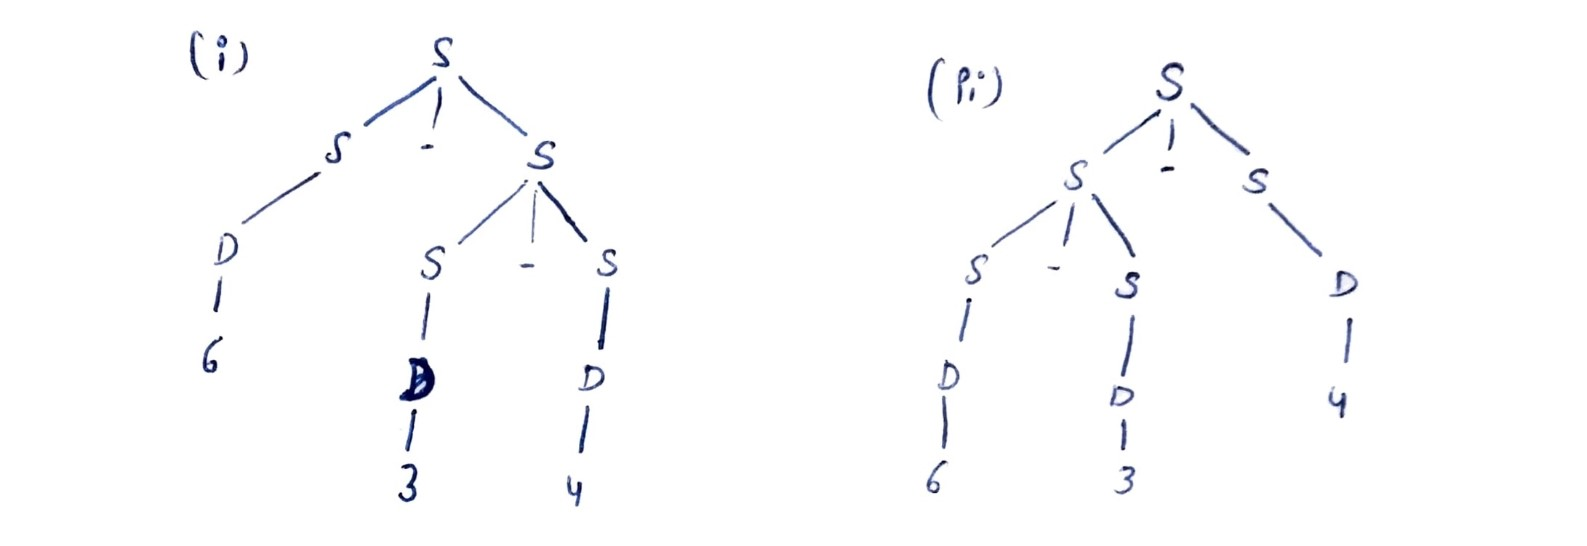
\includegraphics[scale = 0.25]{4.2}
    
    \item This derivation can continue indefinitely, as there is no rule to reduce the expression to a single number. Therefore, "9 - 1 -" is not a well-formed expression according to this grammar.
    
    \item $ S \rightarrow S - S $
    
    $ S \rightarrow S + S - S $

    $ S \rightarrow S + D - S $

    $ S \rightarrow S + S + 3 - D $

    $ S \rightarrow D + D + 3 - 5 $

    $ S \rightarrow 8 + 6 + 3 - 5 $

    \item There are multiple leftmost \& rightmost derivations for this string as the grammar is ambiguous.

    Leftmost derivations are those that start at the root of the parse tree and go down the tree towards the leaves, replacing the leftmost non-terminal symbol with its expansion at each step.
    
    Rightmost derivations are those that start at the leaves of the parse tree and go up the tree towards the root, replacing the rightmost non-terminal symbol with its expansion at each step.
    
    For example, the $2$ leftmost derivations would be:

    \begin{multicols}{2}      
    
    $ S \rightarrow S - S $

    $ S \rightarrow S + S - S $

    $ S \rightarrow S + S + S - S $

    $ S \rightarrow D + S + S - S $

    $ S \rightarrow 8 + D + S - S $

    $ S \rightarrow 8 + 6 + D - S $

    $ S \rightarrow 8 + 6 + 3 - D $

    $ S \rightarrow 8 + 6 + 3 - 5 $


    $ S \rightarrow S + S $

    $ S \rightarrow D + S $

    $ S \rightarrow 8 + S + S $

    $ S \rightarrow 8 + D + S $

    $ S \rightarrow 8 + 6 + S - S $

    $ S \rightarrow 8 + 6 + D - S $

    $ S \rightarrow 8 + 6 + 3 - D $

    $ S \rightarrow 8 + 6 + 3 - 5 $

    \end{multicols}
\end{enumerate}




% PROBLEM 5
\newproblem 
\begin{enumerate}

    \item
    
    \item
    
    \item Yes, the grammar is ambiguous because there are multiple parse trees possible.
    
    \item $ S \rightarrow  S + T \mid T $
    
    $ T \rightarrow T - F \mid F $

    $ F \rightarrow D \mid \epsilon $

    \item Yes. We can control the precedence of $'+'$ and $'-'$ signs. The grammar in $5.4$ gives $'-'$ sign precedence over $'+'$. Other way is to give precedence to $'+'$.

\end{enumerate}

% PROBLEM 6
\newproblem
\begin{enumerate}

    \item $ S \rightarrow DS \mid ,X \mid \epsilon $
    
    $ X \rightarrow DS $

    $ D \rightarrow 0 \mid 1 \mid 2 \mid 3 \mid 4 \mid 5 \mid 6 \mid 7 \mid 8 \mid 9 $
    
    It is unambiguous because the grammar is right recursive and right associated.

    \item 


\end{enumerate}

\end{document}